\documentclass[varwidth=true, border=2pt]{standalone}
\usepackage{tikz}
\usepackage{tqft}

\begin{document}
    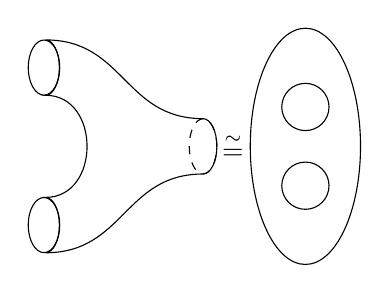
\begin{tikzpicture}[tqft/flow=east]
        \node[tqft/pair of pants,draw,rotate=-180] (a) {};
        \draw (-1.02,-1) ellipse (0.2cm and 0.35cm);
        \draw (-1.02,+1) ellipse (0.2cm and 0.35cm);
        \draw[dashed] (1,0) ellipse (0.175cm and 0.35cm);

        \draw (2.3,0) ellipse (0.7cm and 1.5cm);
        \draw (2.3,+0.5) circle (0.3cm);
        \draw (2.3,-0.5) circle (0.3cm);

        \node at (1.38,0) {$\stackrel{\sim}{=}$};
    \end{tikzpicture}
\end{document}
